\documentclass[journal]{vgtc}                % final (journal style)
%\documentclass[review,journal]{vgtc}         % review (journal style)
%\documentclass[widereview]{vgtc}             % wide-spaced review
%\documentclass[preprint,journal]{vgtc}       % preprint (journal style)

%% Uncomment one of the lines above depending on where your paper is
%% in the conference process. ``review'' and ``widereview'' are for review
%% submission, ``preprint'' is for pre-publication, and the final version
%% doesn't use a specific qualifier.

%% Please use one of the ``review'' options in combination with the
%% assigned online id (see below) ONLY if your paper uses a double blind
%% review process. Some conferences, like IEEE Vis and InfoVis, have NOT
%% in the past.

%% Please use the ``preprint''  option when producing a preprint version
%% for sharing your article on an open access repository

%% Please note that the use of figures other than the optional teaser is not permitted on the first page
%% of the journal version.  Figures should begin on the second page and be
%% in CMYK or Grey scale format, otherwise, colour shifting may occur
%% during the printing process.  Papers submitted with figures other than the optional teaser on the
%% first page will be refused. Also, the teaser figure should only have the
%% width of the abstract as the template enforces it.

%% These few lines make a distinction between latex and pdflatex calls and they
%% bring in essential packages for graphics and font handling.
%% Note that due to the \DeclareGraphicsExtensions{} call it is no longer necessary
%% to provide the the path and extension of a graphics file:
%% 
\includegraphics{diamondrule} is completely sufficient.
%%
\ifpdf%                                % if we use pdflatex
  \pdfoutput=1\relax                   % create PDFs from pdfLaTeX
  \pdfcompresslevel=9                  % PDF Compression
  \pdfoptionpdfminorversion=7          % create PDF 1.7
  \ExecuteOptions{pdftex}
  \usepackage{graphicx}                % allow us to embed graphics files
  \DeclareGraphicsExtensions{.pdf,.png,.jpg,.jpeg} % for pdflatex we expect .pdf, .png, or .jpg files
\else%                                 % else we use pure latex
  \ExecuteOptions{dvips}
  \usepackage{graphicx}                % allow us to embed graphics files
  \DeclareGraphicsExtensions{.eps}     % for pure latex we expect eps files
\fi%

%% it is recomended to use ``\autoref{sec:bla}'' instead of ``Fig.~\ref{sec:bla}''
\graphicspath{{figures/}{pictures/}{images/}{./}} % where to search for the images

\usepackage{microtype}                 % use micro-typography (slightly more compact, better to read)
\PassOptionsToPackage{warn}{textcomp}  % to address font issues with \textrightarrow
\usepackage{textcomp}                  % use better special symbols
\usepackage{mathptmx}                  % use matching math font
\usepackage{times}                     % we use Times as the main font
\renewcommand*\ttdefault{txtt}         % a nicer typewriter font
\usepackage{cite}                      % needed to automatically sort the references
\usepackage{tabu}                      % only used for the table example
\usepackage{booktabs}                  % only used for the table example
%% We encourage the use of mathptmx for consistent usage of times font
%% throughout the proceedings. However, if you encounter conflicts
%% with other math-related packages, you may want to disable it.

%% In preprint mode you may define your own headline. If not, the default IEEE copyright message will appear in preprint mode.
%\preprinttext{To appear in IEEE Transactions on Visualization and Computer Graphics.}

%% In preprint mode, this adds a link to the version of the paper on IEEEXplore
%% Uncomment this line when you produce a preprint version of the article 
%% after the article receives a DOI for the paper from IEEE
%\ieeedoi{xx.xxxx/TVCG.201x.xxxxxxx}

%% If you are submitting a paper to a conference for review with a double
%% blind reviewing process, please replace the value ``0'' below with your
%% OnlineID. Otherwise, you may safely leave it at ``0''.
\onlineid{0}

% custom includes, not part of template:
\usepackage{minted}% syntax highlighting
\usepackage{verbatim}
\usepackage[dvipsnames]{xcolor}

%% declare the category of your paper, only shown in review mode
\vgtccategory{Research}
%% please declare the paper type of your paper to help reviewers, only shown in review mode
%% choices:
%% * algorithm/technique
%% * application/design study
%% * evaluation
%% * system
%% * theory/model
\vgtcpapertype{please specify}

\newcommand{\makeSampleFig}{%
\begin{figure}[tb]
 \centering % avoid the use of \begin{center}...\end{center} and use \centering instead (more compact)
 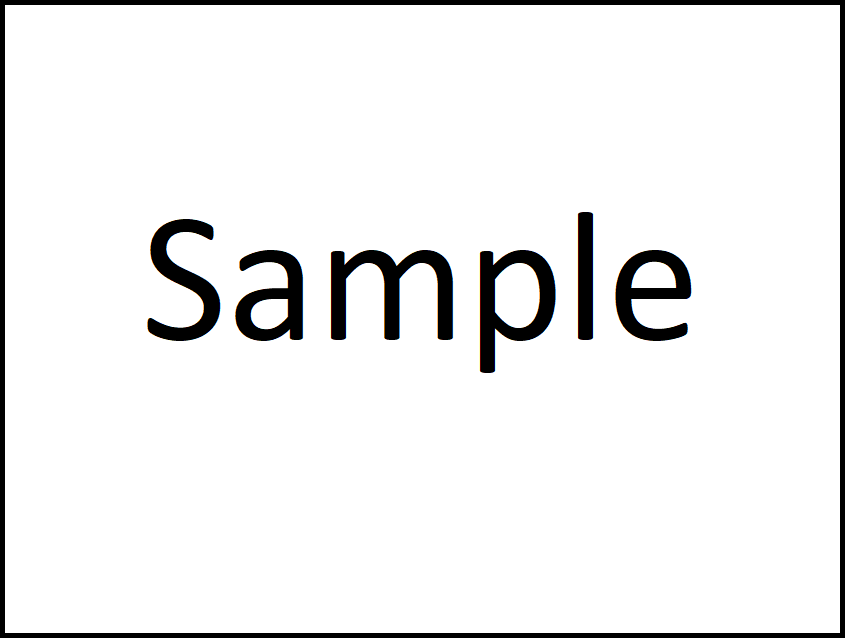
\includegraphics[width=\columnwidth]{sample}
 \caption{A visualization of the 1990--2015 data from \autoref{tab:vis_papers}. The image is from \cite{Isenberg:2017:VMC} and is in the public domain.}
 \label{fig:sample}
\end{figure}}

\newcommand{\makeBasicPlottingFig}{%
\begin{figure*}[!btp]
 \centering
% \includegraphics[width=\linewidth]{basicPlotting}
 \includegraphics[width=1.0\textwidth]{figures/basicPlotting.pdf}
 \caption{A selection of basic plots from PyQtGraph's suite of examples.}
 \label{fig:basicPlotting}
\end{figure*}}

\newcommand{\makePtreeExFig}{%
\begin{figure}[!htbp]
\centering
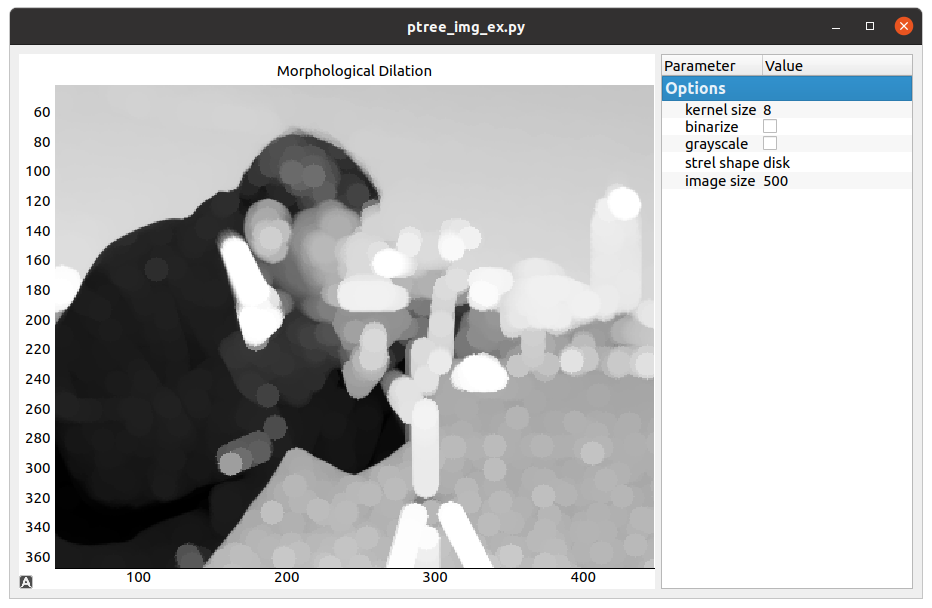
\includegraphics[width=\columnwidth]{figures/pg_ptree_ex}
\caption{Sample use case of parameter trees for function interaction, where various image processing parameters can be quickly updated. Of note, the displayed image reflects these changes in real-time.}
 \label{fig:ptreeEx}
\end{figure}}

\newcommand{\makeLineBenchmarkFig}{
\begin{figure}[!b]
\centering
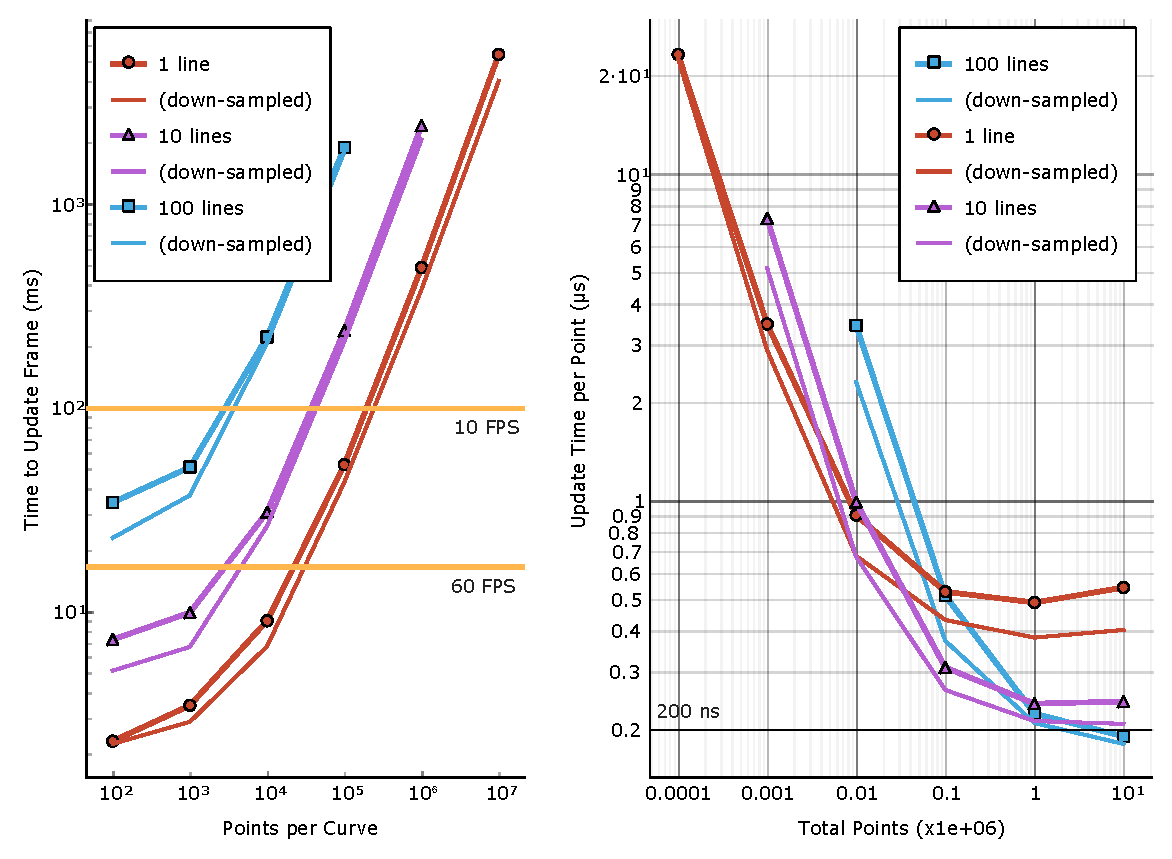
\includegraphics[width=\columnwidth]{figures/lineBenchmark}
\caption{Line speed benchmark. The time to render 1, 10 or 100 lines of data is shown for varying numbers of points per line. All data was collected on a 2020 MacBook Pro with i5 Processor. Left: Time per update over points per curve. The thresholds for achieving 10 and 60 frames/s are shown by horizontal lines. Right: Update time per point, plotted over the total number of points. For more than 100,000 points, the line-plotting time becomes dominant, and the results converge to 200\,ns per point for both 10 and 100 curves, while plotting all points as a single curve increases the time to 500--600 ns\,per point.}
 \label{fig:lineSpeed}
\end{figure}}
 %13-inch 
 
\newcommand{\makeMatplotlibComparison}{%
\begin{figure*}[!bt]
\centering
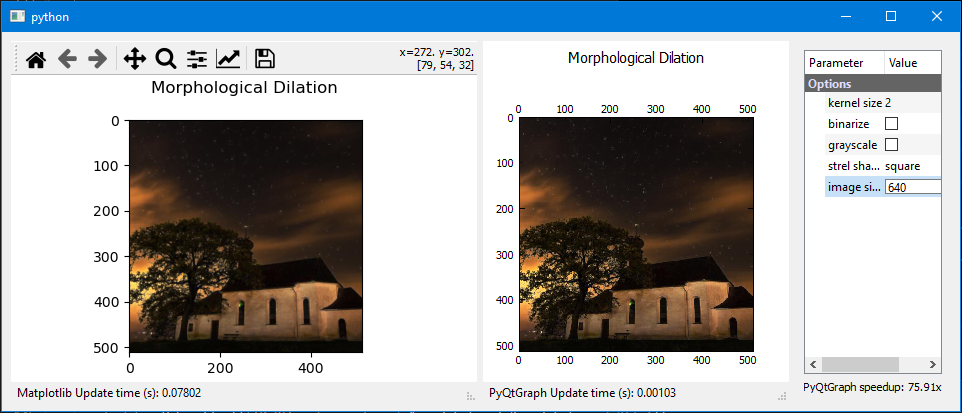
\includegraphics[width=0.8\textwidth]{figures/pg-mpl-comparison}
\caption{Performance test with PyQtGraph and Matplotlib widgets embedded in a Qt5 application. Over a wide range of image sizes, PyQtGraph completes drawing approximately 75--150 times faster, even without hardware acceleration. }
 \label{fig:mpl}
\end{figure*}}

\newcommand{\makeMonitoringFig}{%
\begin{figure}[!htbp]
\centering
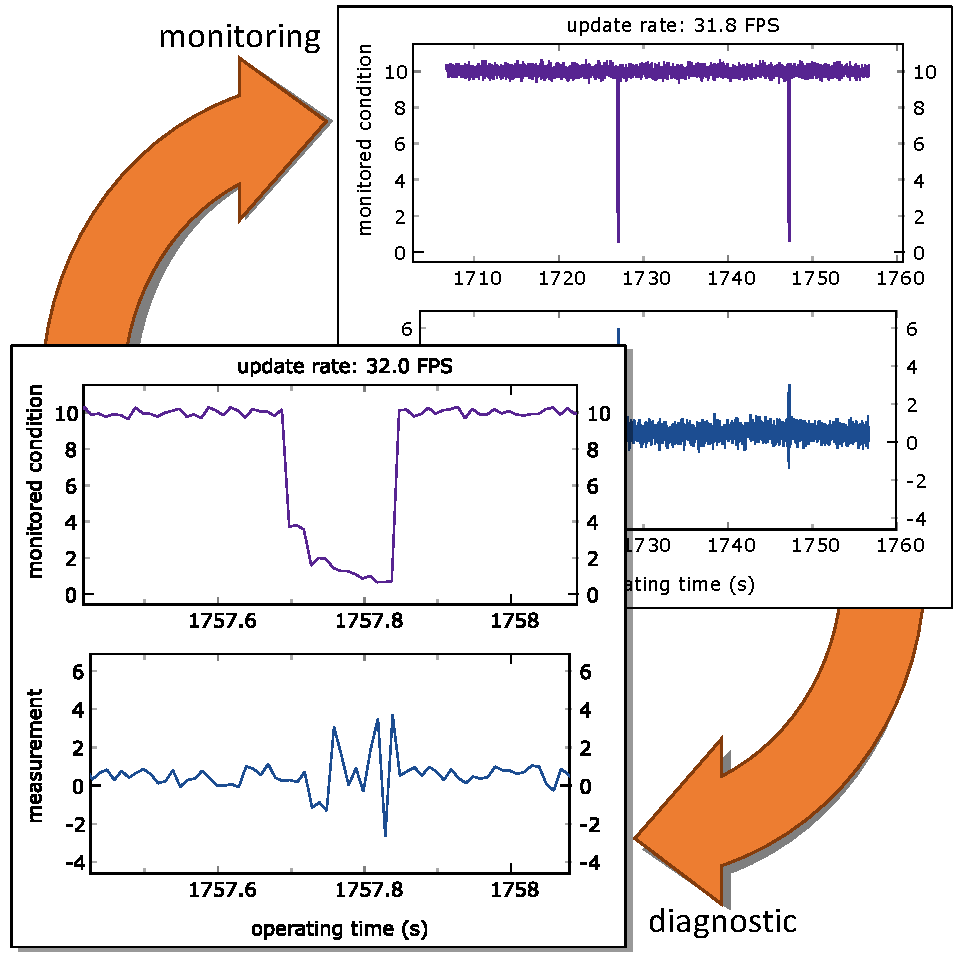
\includegraphics[width=\columnwidth]{figures/monitoring_example_vector.pdf}
\caption{Monitoring and diagnostic of a (simulated) experiment with intermittent failures. Incoming data at 100 samples/s for two measurement channels is recorded into a rolling 5,000 point buffer and continuously displayed at 30 frames/s. When a failure is observed, it can quickly be brought into focus with simple mouse interactions (click-and-drag and mousewheel zoom) for inspection, or to record accurate time stamps. Afterwards, a single click returns the view to automatic scaling without loss of any incoming data.}
 \label{fig:monitoring}
\end{figure}}


%% Paper title.
\title{PyQtGraph - High Performance Visualization for All Platforms}

%% This is how authors are specified in the journal style

%% indicate IEEE Member or Student Member in form indicated below
\author{Ognyan Moore, Luke Campagnola, Martin Chase, Nils Nemitz, and Nathan Jessurun}
\authorfooter{
%% insert punctuation at end of each item
\item Ognyan Moore is with Sensory Inc. E-mail: ognyan.moore@gmail.com.
\item Luke Campagnola is with the Allen Institute.  E-mail: lukec@alleninstitute.org
\item Martin Chase is independent.  E-mail: outofculture@gmail.com.
\item Nils Nemitz is independent. E-mail: nils.nemitz@gmx.de
\item Nathan Jessurun is with the University of Florida. E-mail: njessurun@ufl.edu.
}

%other entries to be set up for journal
\shortauthortitle{Biv \MakeLowercase{\textit{et al.}}: High performance interactive visualizations}
%\shortauthortitle{Firstauthor \MakeLowercase{\textit{et al.}}: Paper Title}

%% Abstract section.
\abstract{

PyQtGraph is a plotting library with high performance, cross-platform support and interactivity as its primary objectives. These goals are achieved by connecting the Qt GUI framework and the scientific Python ecosystem. The end result is a plotting library that supports the use of python and NumPy arrays to drive interactive visualizations on all major operating systems.

Whereas most scientific visualization tools for Python are oriented around publication-quality plotting and browser-based user interaction, PyQtGraph occupies a niche for applications in data analysis and hardware control that require real-time visualization and interactivity in a desktop environment. 

The well-established framework supports line plots, scatter plots, and images, including time-series 3D data represented as 4D arrays, in addition to the basic drawing primitives provided by Qt.

For datasets up to several hundred thousand points, real-time rendering speed is achieved by optimized interaction with the Python bindings of the Qt framework. For enhanced image processing capabilities, PyQtGraph optionally integrates with CUDA. This ensures rendering capabilities are scalable with increasing data demands. Moreover, this improvement is enabled simply by installing the CuPy library, i.e. requiring no in-depth user configurations.

PyQtGraph provides interactivity not only for panning and scaling, but also through mouse hover, click, drag events and other common native interactions. Since PyQtGraph uses the Qt framework, the user can substitute their own intended application behavior to those events if they feel the library defaults are not appropriate.  This flexibility allows the development of customized and streamlined user interfaces for data manipulation.

% Furthermore, the parameter tree framework for developers to provide simple data selection and manipulation.)) 

The included parameter tree framework allows straightforward interactions with arbitrary user functions and configuration settings. Callbacks execute on changing parameter values, even asynchronously if requested.

An active developer community and regular release cycles indicate and encourage further library development. PyQtGraph's support cycle is synchronized with the NEP-29 standard, ensuring most popular scientific python modules are continually compatible with each release.


PyQtGraph is available through pypi.org (\href{https://pypi.org/project/pyqtgraph/}{https://pypi.org/project/pyqtgraph/}), conda-forge ({\href{https://anaconda.org/conda-forge/pyqtgraph}{https://anaconda.org/conda-forge/pyqtgraph}}) and GitHub (\href{https://github.com/pyqtgraph/pyqtgraph}{https://github.com/pyqtgraph/pyqtgraph}).%
} % end of abstract

%% Keywords that describe your work. Will show as 'Index Terms' in journal
%% please capitalize first letter and insert punctuation after last keyword
\keywords{Visualization, NumPy, PyData, Python}

%% ACM Computing Classification System (CCS). 
%% See <http://www.acm.org/class/1998/> for details.
%% The ``\CCScat'' command takes four arguments.

\CCScatlist{ % not used in journal version
 \CCScat{K.6.1}{Management of Computing and Information Systems}%
{Project and People Management}{Life Cycle};
 \CCScat{K.7.m}{The Computing Profession}{Miscellaneous}{Ethics}
}

%% A teaser figure can be included as follows
\teaser{
  \centering
  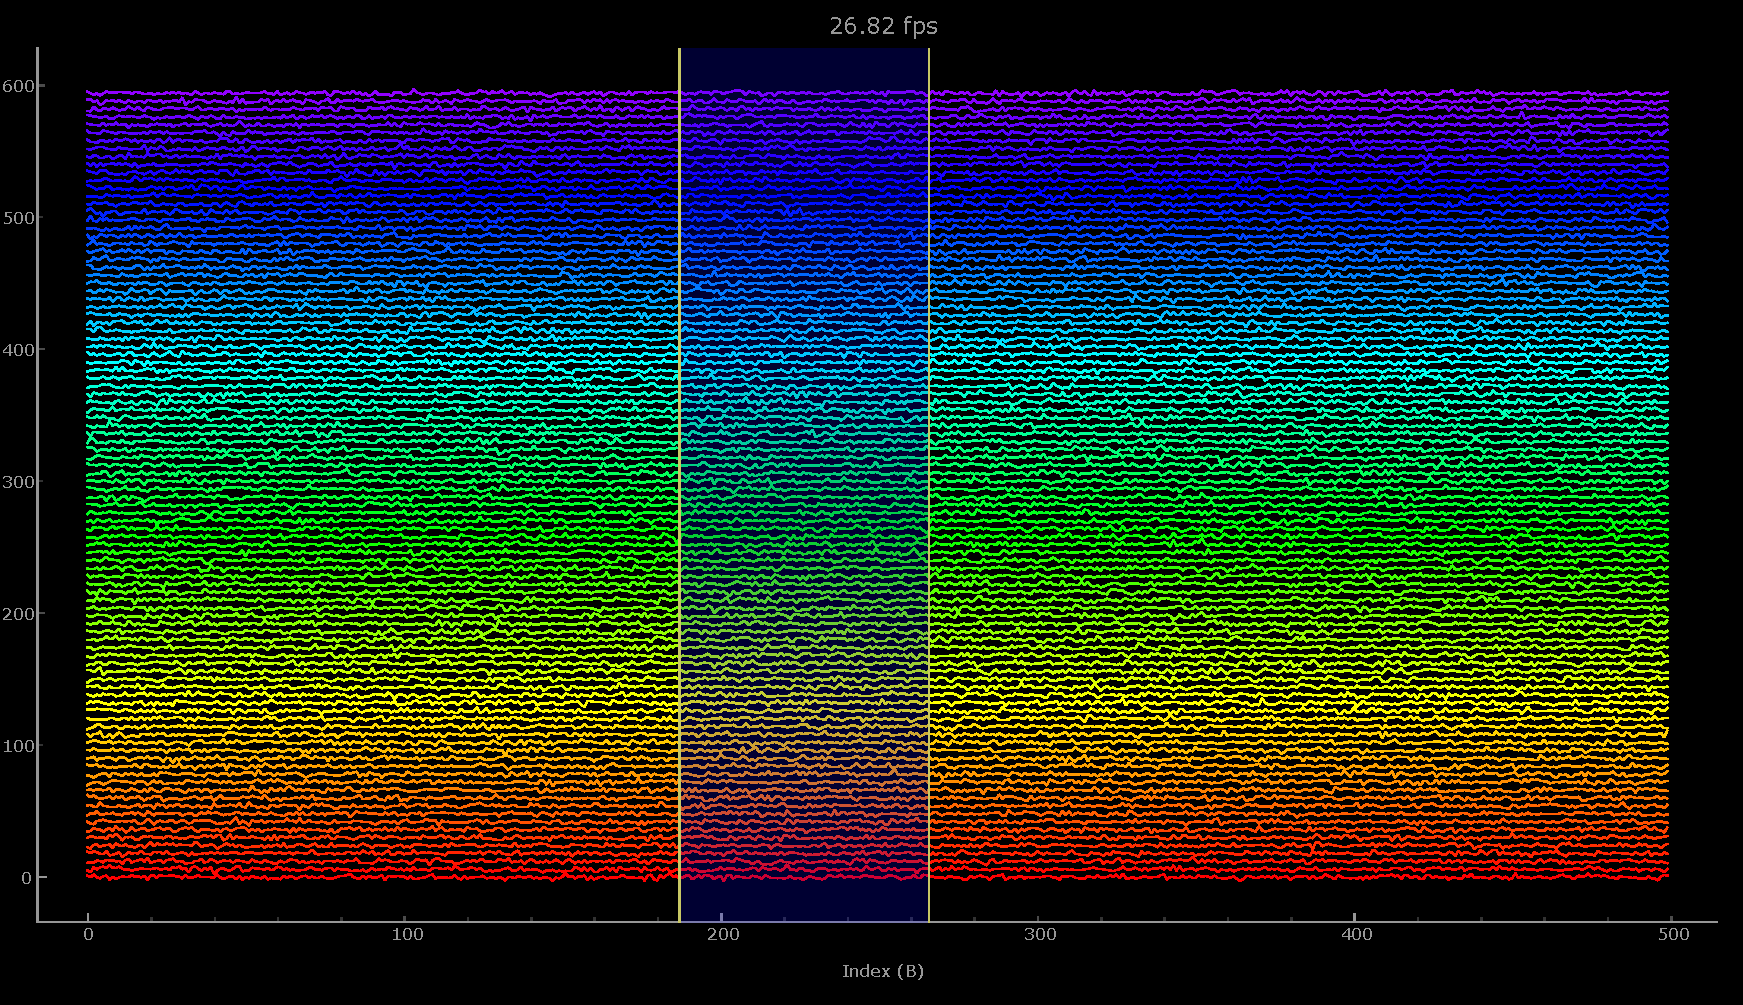
\includegraphics[width=\linewidth]{multiplot}
  \caption{Screenshot of interactive plot widget with 100 lines each containing 500 points}
  \label{fig:teaser}
}

%% Uncomment below to disable the manuscript note
%\renewcommand{\manuscriptnotetxt}{}

%% Copyright space is enabled by default as required by guidelines.
%% It is disabled by the 'review' option or via the following command:
% \nocopyrightspace


\vgtcinsertpkg

%%%%%%%%%%%%%%%%%%%%%%%%%%%%%%%%%%%%%%%%%%%%%%%%%%%%%%%%%%%%%%%%
%%%%%%%%%%%%%%%%%%%%%% START OF THE PAPER %%%%%%%%%%%%%%%%%%%%%%
%%%%%%%%%%%%%%%%%%%%%%%%%%%%%%%%%%%%%%%%%%%%%%%%%%%%%%%%%%%%%%%%%

\begin{document}

%% The ``\maketitle'' command must be the first command after the
%% ``\begin{document}'' command. It prepares and prints the title block.

%% the only exception to this rule is the \firstsection command
\firstsection{Introduction}
% Nils and Ogi
\maketitle

The benefits of interactive exploration of scientific data were recognized as soon as computer systems gained graphical displays. While early implementations like the PRIM-9 system\cite{prim9} of the Stanford Linear Accelerator Center were only available to large installations, more affordable microcomputers soon found their place in smaller laboratories also\cite{Byrd79}\cite{Reed80}, controlling experiments and recording data.

Software packages designed to acquire and process this data soon appeared, with MATLAB\cite{matlab} and LabView\cite{labview} both implementing graphical representation of data from their very first versions. The latter was designed to enable data acquisition, processing and visualization all in the framework of a single program. This approach remains common in fields like statistics where the tools for interaction with data are reasonably well-defined. In other areas, the advent of high-level programming languages like Java and Python has enabled researchers to create the tools for their specific needs with reasonable time investment. This is facilitated by a continuously growing open-source infrastructure that provides resources addressing anything from mathematical methods\cite{numpy2020} to full-scale laboratory data infrastructure\cite{Johnson2015, Koerner2019}.

With less need to recreate existing solutions, it becomes feasible to implement software aiming to reduce turn-around times of iterated experiments: A traditional view of the scientific method envisions a sequence of detailed experiment design, pain-staking note-taking, followed by an exhaustive evaluation resulting in a revised experiment. However, when experiments can be optimized over a wide parameter space, the evaluation quickly becomes the dominant factor. Even for established experimental parameters, external factors such as degraded performance of equipment result in a significant loss of time if they are discovered only in subsequent evaluation.

The solution is to provide immediate feedback to the researcher throughout the experiments, and data visualization has long proven its effectiveness in this regard [Friendly2008]. A challenge lies in providing tools for a detailed inspection of interesting data while new information continues to arrive at rates that for extreme cases are counted in Gb/s even after preselection\cite{LHC}. These tools also need to provide the flexibility to handle data that falls outside the range expected in design, as this is the most likely to indicate failures or to provide the sought-after discovery.

Here we present a visualization library created with these goals in mind. Although written in Python to allow for easy expansion, a close integration with the cross-platform Qt UI framework\cite{Qt} it provides the capability to interactively handle datasets of hundreds of thousands of points, or live representation of high-resolution camera data.


\section{Approach}
\subsection{Python}
The Python programming language enjoys a large popularity in scientific research due ease of entry and a robust standard library combined with access to very comprehensive numerical computing packages. This makes Python an attractive alternative to established computational tools such as MATLAB\cite{matlab} and Mathematica. %[mathematica].  

The set of most commonly used scientific computing tools in Python are commonly referred to as the SciPy stack. % I think this is still true :)
This refers to SciPy, NumPy, and a variety of other libraries that use the NumPy \texttt{ndarray} data structure as a container for vectorized operations. The \texttt{ndarray} gives developers a high level API to low-level operations with excellent performance. This API allows NumPy and SciPy to provide a wide variety of standard numerical computing operations, all of which are very efficient and help overcome the performance penalty of working with Python as a cross-platform, interpreted, dynamically typed language.

\subsection{Qt}
The Qt framework is a GUI platform written in C++ that allows the creation of cross-platform applications with a single shared code-base. Comprehensive Python bindings (PyQt) expose the complete Qt API. Here, the specific section of interest is the \texttt{GraphicsView} framework, which provides a surface for managing and interacting with a large number of custom-made 2D graphical items, with support for zooming and rotation\cite{QtGraphicsView}. PyQtGraph is built on this foundation to extend the SciPy stack with performant cross-platform visualization.

\subsection{Implementation}
\texttt{GraphicsView} renders line segments in a freely scaled coordinate system through \texttt{QPainterPath} objects. The rendering performance of PyQtGraph results from optimized code to create such paths directly from NumPy ndarrays describing sets of $x$ and $y$ coordinates. The core function \texttt{arrayToQPath} uses NumPy's structured array functionality to efficiently create a binary compatible structure that can serve as an input stream to a \texttt{QPainterPath} item (see Appendix \ref{app_arrayToQPath}). This \texttt{QPainterPath} is then drawn to the screen by the Graphics View framework.


\color{brown}
\section{Effective Methods}
\subsection{Python}

% First off, I'm going to say, my paragraphs are absolutely terrible compared to the Introduction Nils wrote, so please keep this in mind as you read below.

% TODO: remove all references to SciPy stack as it's considered obsolete per: https://scipy.org/stackspec.html

The Python programming language has gained in popularity in a variety of fields, but especially so in scientific research.  This rise in popularity is due to many factors, such as ease of entry, robust standard library, and accessibility to very comprehensive numerical computing libraries.  This low barrier of entry, combined with being free and open source as well as the numerical computing libraries available make Python an attractive alternative to other established programming tools such as MATLAB[matlab] and Mathematica[mathematica].  

A set of very highly used libraries used for scientific computing in Python is referred to the SciPy stack.  These libraries refer to NumPy, SciPy, and a variety of other libraries that use the NumPy \texttt{ndarray} data structure that acts as a container for which vectorized operations can applied on.  The \texttt{ndarray} provides Python developers with a high level API to interact with the ndarrays, but the operations are happening on a very low level, so the performance is quite good.  The API for NumPy and SciPy provide developers with access to a wide variety of standard numerical computing operations, all of which are very efficient.

There are another set of python libraries, that for the purposes of this paper are interchangeable, collectively referred to as python Qt-bindings, or PyQt.  These libraries provide a python interface to the Qt framework[qt].  The Qt framework is a GUI framework written in C++ allowing developers to create applications that work on all major desktop operating systems using a single code-base.  The Python Qt bindings give that same capability to python developers; emulating the C++ API.  The Qt framework is quite expansive, and covers everything one can think would be needed for a integration into the operating system or the display of standard widgets such as text fields, labels, drop downs and so on.  A specific section within the Qt framework of interest to us is the Graphics View framework.  "Graphics View provides a surface for managing and interacting with a large number of custom-made 2D graphical items, and a view widget for visualizing the items, with support for zooming and rotation."  <note, this is the quote verbatim, I have no problem sourcing it or would it be more beneficial to word it?>. Graphics View, which is included as part of PyQt provides us the low-level efficient API to draw content on a screen that can be resized, scaled, which is just what is needed for data visualization.  

What PyQtGraph does is bridge the gap from the SciPy stack to the Graphics View framework with the Qt library.  This provides python developers a way to manipulate and display large data quantities at very fast and efficient scales, into applications that are cross-platform compatible, while remaining in the Python ecosystem.


SciPy Stack
https://scipy.org/stackspec.html

Graphics View:
https://doc.qt.io/qt-5/graphicsview.html

\color{black}
\section{Capabilities}

All 2d rendering functions that handle large quantities of data are implemented on top of the \texttt{arrayToQPath} conversion. These cover all common plotting requirements. Figure~\ref{fig:basicPlotting} shows a demonstration from PyQtGraph's suite of examples.

\subsection{Plot Types}
\makeBasicPlottingFig

PyQtGraph shows all plots within a \texttt{PlotItem} object consisting of a \texttt{ViewBox} equipped with a set of axes. This allows dynamic pan and zoom through the transforms of Qt's \texttt{GraphicsView}, with no need to regenerate the \texttt{QPainterPath} objects. Individual elements of the plot are represented by graphics items that share the same coordinate systems and shown in any combination and drawing order. 

PyQtGraph represents line plots as \texttt{PlotCurveItem} objects and offers typical functionality such as color, width and dashing. "Shadow pen" lines can be underlaid for additional contrast. 

Scatter plot items are assigned a default shape, color and size per data set, but each point can also have a unique attributes. Shapes are pre-rendered and cached to optimize performance when the underlying dataset is updated. Depending on the application, symbols can be set to scale with the view or maintain constant size.  Functionality is included for items in scatter plots to recognize mouse hover events.

%An error bar plot is provided that handles $x$, $y$ coordinates, height, width, and lengths in any direction for lines representing errors.  
Plots can be extended by both horizontal and vertical error bars and annotated by text labels. Built in routines can also transform the plotted data to provide logarithmic scaling, Fourier transforms, and to show the gradient $dy/dt$ directly over $t$ or as a phase map over $y$.

Bar graphs and images also make use of this framework and can be added to the same PlotItem, although they are more commonly used separately. Users can also create \texttt{QPainterPath} objects to add their own graphical elements using the well documented methods of the Qt Graphics View framework. PyQtGraph's suite of examples\cite{pg_examples} illustrates this with some demonstrations.

\color{brown}
\subsubsection{Performance}

PyQtGraph makes heavy use of the Graphics View framework within Qt [graphicsview] to handle drawing, scaling, and the managing coordinate systems.  To render line paths in the Graphics View framework, \texttt{QPainterPath} objects are added to the view.  PyQtGraph has some heavily optimized functions for creating \texttt{QPainterPaths} from NumPy \texttt{ndarray} objects.  The function, \texttt{arrayToQPath} takes in two \texttt{ndarray} objects of the same length, the first representing x-coordinates, and the second representing y-coordinates. First thing that is done is create a NumPy structured array composed of fields, $c$, $x$, and $y$.  The $c$ field corresponds to if this element should be connected to a line, and the $x$ and $y$ fields correspond to the coordinate of the point that we wish to connect, or not connect.  From this structured array, we construct a view into this array named byteview, but the datatype of the view is an unsigned integer.  The structured array is then filled up out with the input arrays, with handling for NaN values, and depending on if an optional argument is passed to the function limiting which points get connected.  From byteview, a \texttt{QByteArray} object is created, which is promptly converted to a \texttt{QDataStream} object, which has the contents written to a \texttt{QPainterPath} item.  This \texttt{QPainterPath} item is then drawn directly by the Graphics View framework onto the screen.

The reason this is fast is that this performed so well is that the data was copied once into the structured array from generic NumPy ndarrays, and from then it was just referenced during the creation of the other C++ objects, before eventually resulting in the creation of an object that could be rendered.

\color{black}
\subsection{Images and Regions of Interest}

PyQtGraph provides the means to display images and other matrix-like data. Handling streams of such data, as in live video, is also enabled by efficient NumPy methods that convert the input data into a binary representation that can be used directly by the Qt framework. Various analysis and processing tools can be used to alter the image arrays, such as look-up tables (LUT) for color-mapped display, region of interest (ROI) and histograms.

\subsubsection{Image Views}

The principal object in displaying images, \texttt{ImageItem}, accepts 2-dimensional (interpreted as greyscale) or 3-dimensional (either RGB or RGBA) data of any numeric type. This input is then processed and converted into Qt's \texttt{QImage} format for rapid display. Customized LUTs can be applied for colormap alterations. An associated \texttt{HistogramLUTWidget} object can optionally provide both a useful analysis tool and a means of automatically or interactively scaling the image data.

\subsubsection{ROIs}
A common image analysis task is to define a region of interest (ROI) in a larger original image. This is supported by multiple interactive objects (\texttt{LineROI}, \texttt{CircleROI}, \texttt{PolygonROI}, and others), which provide NumPy slice objects that reference the selected region within the image array. Once extracted, the relevant data can then be further processed. Magnification, live plotting and custom analysis are all simple to implement. Multiple ROIs can be used together to provide background correction or plot comparisons. These ROI objects remain interactive while attached to the image, so that resizing, moving and rotating a ROI can prompt immediate updates of all subsequent plotting and analysis interfaces.

\color{Black}
\subsubsection{Performance}
% Martin - discuss makeqimage, also a good opportunity to discuss CUDA support



%\subsection{Custom Graphics}

%Since PyQtGraph uses the Graphics View framework there is nothing limiting users to the plot types that PyQtGraph offers.  End users are able to create their own \texttt{QPainterPath} objects, with brush and pen options that they desire, draw the shapes they want in the position they want.  The Qt documentation is quite extensive on the subject and PyQtGraph provides an example of some custom plots of this nature in the example application.

\subsection{Interactivity}

\color{DarkOrchid}
\subsubsection{Event Driven GUI}
The Qt framework is event driven, which enables PyQtGraph to provide seamless mouse interaction, but also allows users to develop their own desired behavior from mouse move, hover, leave, enter, double-click, zoom, or drag events. Almost every aspect of PyQtGraph interacts with the Qt events, or provides its own in response to e.g. axis adjustments or changes to a selected region. This interactivity is a core component of the Qt framework, and adding such behavior to a plot in PyQtGraph is no more complicated than generating the plot in the first place.

\subsubsection{Responsiveness at scale}

Recognizing zoom events enables resolution-aware downsampling of the plotted data. Multiple available methods provide different trade-offs of accuracy against performance, and include a "peak" display that precisely captures the minima and maxima of the data, a "mean" over the downsampled interval, and a fast "subsample" that displays only 1 in N datapoints. Automatic downsampling allows responsive display of large datasets, where zooming in automatically reveals more detail.



\color{brown}
\subsubsection{Event Driven GUI}

The Qt framework is event driven, meaning developers can make their application react to various events seamlessly.  This capability allows for PyQtGraph to provide seamless mouse interaction, or allow users to develop their own desired behavior from mouse move, hover, leave, enter, double-click, zoom, or drag events.  Almost every aspect of PyQtGraph interacts with these events that the Qt framework emits when appropriately.  There are some common use-cases that developers may want to have, such as synchronizing the axes of multiple plots, or being able to select a region of a plot.  As this interactivity is a core component of the Qt framework, adding this interactivity to a plot in PyQtGraph is no more complicated than generating the plot in the first place.

\subsubsection{Responsiveness at Scale} % / scalable responsiveness / real-time data crunching / plots go brrrr

Recognizing zoom events, combined with knowledge of the number of pixels in the plot area, allows for significant performance benefits involving down-sampling.  As PyQtGraph recognizes the number of pixels on the screen, and the number of data plots a user is trying to plot, PyQtGraph is capable of down-sampling the displayed data in a variety of ways should the user request it.  The methods provides are subsampleing, where the first of N samples are plotted, "mean", where an average of N samples are plotted, and "peak" where a vertical line between the maximum and minimum of N samples is drawn.  Each method has its own performance considerations, but this kind of automatic down-sampling allows for significant performance improvements when plotting data represented in large \texttt{ndarray} objects, and more detail is revealed automatically during zoom operations.

\color{red}
Another popular use case is to define sub-regions of plots to show in more detail, and when the sub-region is adjusted, a secondary, linked plot has its view updated to show that particular data.  If a linked-plot has to do some supplemental calculations, for example, displaying a spectrogram from a subset of the data selected above, the Qt framework provides multi-threaded capabilities so that the computation can be done on a separate thread, and the display can be updated when the calculation is complete.  This kind of multi-threaded approach can result in an application with a smooth user experience while also performing significant calculations in the background.

\color{black}

\subsubsection{Parameter Trees}\label{sec:paramtrees}
While automated interaction through mouse and keyboard events are critical for seamless user interaction, a mechanism for injecting custom algorithm parameters, configuration settings, and more can be equally important. PyQtGraph provides this capability through Parameter Trees, which allow groupings of arbitrary user-settable data. These leverage existing Qt widgets for text, numeric, list-like, and custom data types while providing callback hooks for when values change or a certain action is triggered. Callbacks can be registered to plot updates, alert messages, data loading, and much more.

Parameters can be grouped, linked, dynamically instantiated / removed, and reordered as needed. They are also capable of saving/loading their states hierarchically, easily allowing users to generate persistent configuration files. Moreover, since the accessor paradigm for Parameters mimics a Python dictionary, they can function as a drop-in replacement for settings that are currently programmatically modified in the same manner.

Multiple use cases for these Parameter trees are highlighted in \autoref{sec:examples}. Common to each is the minimal amount of boilerplate additions to facilitate integration and simplicity in setup and customization.

% I can add more about flowchart integration / design paradigms here, but I am unsure if it is filler or relevant to the conversation. The main point would be how parameters bridge the gap between automated and manual workflows, easing the transition from testing to a production application

\section{Examples}\label{sec:examples}
% everyone, please put a paragraph/section about a tool you use pyqtgraph for

% \subsection{Human-Updatable Processing Parameters}
\color{DarkOrchid}
\subsection{Rapid iteration of processing parameters}
\color{Black}
In applications such as image processing, real-time feedback for various algorithm parameters can be critical in reducing the exploration space of viable solutions. For instance, it might be difficult to tell the appropriate kernel size for a morphological operation without testing multiple combinations of image types, parameter values, and more. These factors often make fine-tuning a laborious process. In these cases, Parameter trees can interact with callbacks as described in \autoref{sec:paramtrees} to directly integrate the programmer into the testing space. A simple example of this is shown in \autoref{fig:ptreeEx}. For more complex image processing workflows, an optimal combination of multiple values can be determined on a trial basis, saved to a given configuration file, and loaded on demand depending on input image properties.
\makePtreeExFig

\color{DarkOrchid}
\subsection{Monitoring of real-time data}
\makeMonitoringFig
Visualization can provide immediate feedback on measurement results and the operational state of the equipment involved. Figure~\ref{fig:monitoring} shows an application of the opportunities provided by PyQtGraph's interactive facilities in this application. For most applications, no data reduction is necessary to maintain smooth display of a sufficiently large buffer, and no additional code is needed to alternate between monitoring of new data and close inspection of specific events.
\color{black}

\color{DarkOrchid}
\section{Software development}
PyQtGraph is released under the open source MIT license. It is known to run on systems ranging from the Raspberry Pi to IBM's s390x architecture. Development is coordinated by volunteer maintainers, with additional code provided by occasional contributors. A continuous integration system asserts that the codebase passes a suite of tests for different combinations of Qt bindings, Python versions and operating systems. PyQtGraph has adopted NEP-29 \emph{(*citation needed*)} to establish a support timeline for Python and NumPy versions in line with the rest of the Python community and development occurs in close communication with projects such as ACQ4 and Orange3 \emph{(*citation needed*)} that constitute a large part of the user base.

\section{Outlook}
With a growing number of both maintainers and contributors, PyQtGraph is well positioned to take advantage of technological developments. The support of hardware acceleration in recent versions of NumPy has already been used to add CUDA integration to some time-critical code, but there is still plenty of potential for further improvements to performance and capabilities. The growing maturity of the Numba just-in-time compiler \emph{(*citation needed*)} for Python code provides additional opportunities for acceleration beyond what NumPy's array operations can provide.

\color{brown}
\section{Outlook}

The outlook for PyQtGraph is very promising.  From a library management point, over the last two years, the number of outstanding pull requests have dropped approximately 85\%, there are 7 active maintainers, and a growing number of contributors as well.  Our continuous integration system has been expanded to cover a greater combination of supported Qt bindings, python versions and operating systems.  PyQtGraph has adopted NEP-29, a timeline with a suggested support for Python and NumPy versions that is in line with the rest of the PyData community; this allows developers to focus on issues with recent versions of the libraries, and not have to worry about configurations that current PyQtGraph users are unlikely to encounter.  Lastly, greater effort has been placed on user outreach.  The larger projects that use PyQtGraph such as ACQ4 and Orange3 now have a direct line of communication to maintainers outside the issue tracker.  This has already proven beneficial as many workarounds that these libraries have implemented for themselves are able to be merged into the PyQtGraph library itself.

With regards to project capabilities, the outlook is very good as well.  With NumPy adopting NEP-35, optional support for more specialized libraries can be added in without significant changes to the code-base, the same way CuPy/CUDA support was added.  This, in combination with an increasing number of maintainers, many bugfixes and performance improvements have been made, and a more rapid release cycle has been adopted.

\color{black}
%% if specified like this the section will be committed in review mode
\acknowledgments{
The authors wish to thank A, B, and C. This work was supported in part by
a grant from XYZ (\# 12345-67890).}

%\bibliographystyle{abbrv}
\bibliographystyle{abbrv-doi}
%\bibliographystyle{abbrv-doi-narrow}
%\bibliographystyle{abbrv-doi-hyperref}
%\bibliographystyle{abbrv-doi-hyperref-narrow}

\section{Appendix}
\subsection{Implementation of arrayToQPath}
\label{app_arrayToQPath}
The function \texttt{arrayToQPath} is at the core of PyQtGraphs performance and is included here in full to demonstrate the approach\ref{table:arrayToQPath}. 
Execution take two \texttt{ndarray} objects of the same length, representing $x$- and $y$-coordinates for for a series of line segments. Interruptions are relatively rare for the main application of fast line plots, and are represented by interspersed Not-a-Number values. A NumPy structured array composed of fields $c$, $x$, and $y$, where $c$ indicates if a connecting line to this point should be drawn. A NumPy \texttt{view} of this array in \texttt{ubyte} format provides direct memory access. The raw memory structure, wrapped in a \texttt{QByteArray} object, can then be used to initialize a \texttt{QPainterPath} object from a \texttt{QDataStream}. All data conversion is handled by NumPy methods that operate more efficiently on the underlying data structure than is possible from Python itself.

\emph{Comment: I removed}

credit: Divakar https://stackoverflow.com/a/41191127/643629

\emph{from the source. If we want to include that, it should be a citation/comment}


% \begin{verbatim}
\begin{table*}[pht]
\begin{minted}{python}
def arrayToQPath(x, y, connect='all'):
    """Convert an array of x,y coordinats to QPainterPath as efficiently as possible.
    The *connect* argument may be 'all', indicating that each point should be
    connected to the next; 'pairs', indicating that each pair of points
    should be connected, or an array of int32 values (0 or 1) indicating
    connections.
    """
    path = QtGui.QPainterPath()
    n = x.shape[0]
    # create empty array, pad with extra space on either end
    # see: https://github.com/qt/qtbase/blob/dev/src/gui/painting/qpainterpath.cpp
    # All values are big endian--pack using struct.pack('>d') or struct.pack('>i')
    arr = np.empty(n+2, dtype=[('c', '>i4'), ('x', '>f8'), ('y', '>f8')])
    # write first two integers
    byteview = arr.view(dtype=np.ubyte)
    byteview[:16] = 0
    byteview.data[16:20] = struct.pack('>i', n)
    # Fill array with vertex values
    arr[1:-1]['x'] = x
    arr[1:-1]['y'] = y
    # inf/nans internally indicate separate line segments and must be removed for Qt>5.12.3
    isfinite = None
    qtver = [int(x) for x in QtVersion.split('.')]
    if qtver >= [5, 12, 3]:
        isfinite = np.isfinite(x) & np.isfinite(y)
        if not np.all(isfinite):
            mask = ~isfinite
            idx = np.arange(len(x))
            idx[mask] = -1
            np.maximum.accumulate(idx, out=idx)
            first = np.searchsorted(idx, 0)
            if first < len(x):
                # Replace all non-finite entries from beginning of arr with the first finite one
                idx[:first] = first
                arr[1:-1] = arr[1:-1][idx]
    # decide which points are connected by lines
    if eq(connect, 'all'):
        arr[1:-1]['c'] = 1
    elif eq(connect, 'pairs'):
        arr[1:-1]['c'][::2] = 0
        arr[1:-1]['c'][1::2] = 1  # connect every 2nd point to every 1st one
    elif eq(connect, 'finite'):
        if isfinite is None:
            isfinite = np.isfinite(x) & np.isfinite(y)
        arr[2:]['c'] = isfinite
    elif isinstance(connect, np.ndarray):
        arr[2:-1]['c'] = connect[:-1]
    else:
        raise Exception('connect argument must be "all", "pairs", "finite", or array')
    arr[1]['c'] = 0  # the first vertex has no previous vertex to connect

    byteview.data[-20:-16] = struct.pack('>i', 0)  # cStart
    byteview.data[-16:-12] = struct.pack('>i', 0)  # fillRule (Qt.OddEvenFill)

    # create datastream object and stream into path
    path.strn = byteview.data[16:-12]  # make sure data doesn't run away
    try:
        buf = QtCore.QByteArray.fromRawData(path.strn)
    except TypeError:
        buf = QtCore.QByteArray(bytes(path.strn))
    except AttributeError:
        # PyQt6 raises AttributeError
        buf = QtCore.QByteArray(path.strn, path.strn.nbytes)
    ds = QtCore.QDataStream(buf)
    ds >> path
    return path
\end{minted}
\caption{PyQtGraph source code for the core \texttt{arrayToQPath} function.}
\label{table:arrayToQPath}
\end{table*}



\bibliography{template}
\end{document}

